\documentclass[a4paper,12pt]{article}

\usepackage{graphicx}
\usepackage{hyperref}
\usepackage{amssymb}
\usepackage{amsmath}
\usepackage{listings}

\lstset{frame=tb,
  aboveskip=3mm,
  belowskip=3mm,
  columns=flexible,
  basicstyle={\small\ttfamily}
}

\title{Web \& Database Technology --- Summary}
\author{Dany Sluijk}
\date{November 2018}

\makeindex

\begin{document}
\maketitle
\begin{center}
	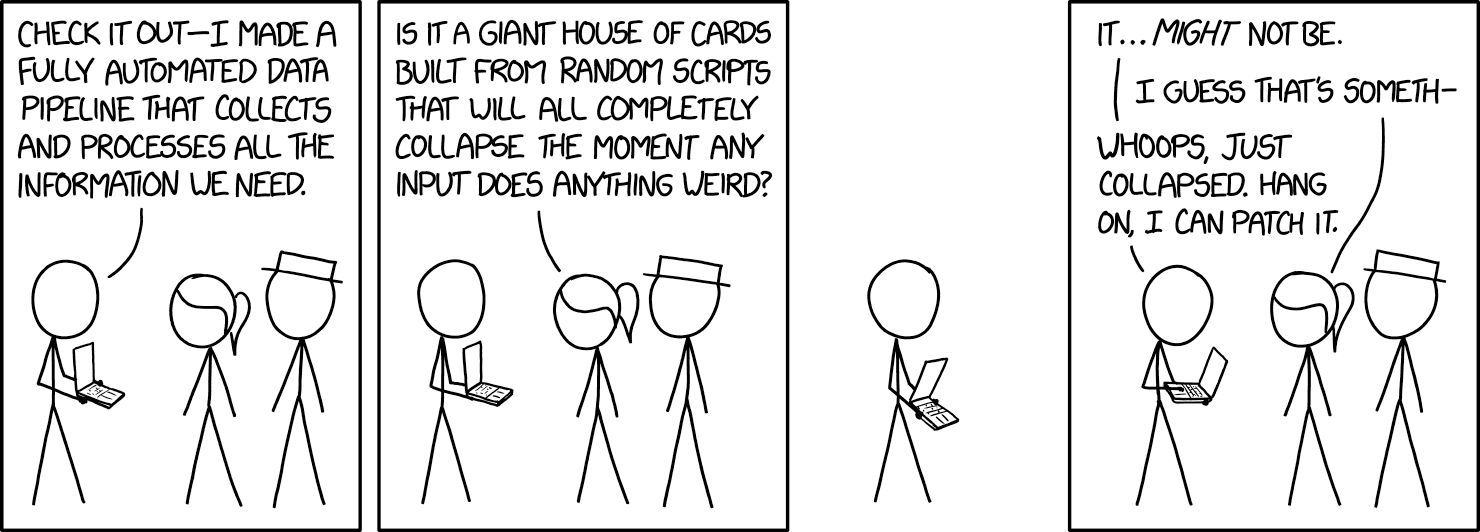
\includegraphics[height=9cm]{./intro}
\end{center}
\begin{abstract}
	This document contains a summary of the Web \& Database Technology course given
	in the first year of Computer Science and Engineering.
	This is \emph{not} a definitive guide, and might contain errors.
	Please send an email to \href{mailto:dany@atlasdev.nl}{``dany@atlasdev.nl''}.
	This summary is distributed under the
	\href{https://opensource.org/licenses/MIT}{MIT} license.
\end{abstract}

\newpage
\tableofcontents

\section{HTTP}
HTTP is one of the most important protocols of the internet.
It's a human readable and text based, making it easy to use.
This summary is talking about version 1.1.
Any other version is out of scope.

\subsection{Protocol}
An example HTTP request looks like the following:

\begin{lstlisting}
POST /say/hello HTTP/1.1
Host: example.com
Content-Length: 12
Content-Type: text/plain
Accept-Encoding: gzip, deflate
Accept-Charset: utf-8
Accept: text/html

Hello world!
\end{lstlisting}

The first line is the {\bf request line}.
It contains the {\bf method} ({\it POST}) and the {\bf path} ({\it /say/hello}).

Moving on we see the first header.
Headers are key-value objects which indicate metadata about the request.
The first one is {\it Host}, which gives which domain you are requesting from.
Together with the request line gives a valid HTTP/1.1 request.

The following five lines are other headers.
More on these headers can be found within the Headers subsection.

The next line is just empty.
This indicates that the headers have come to an end.

After that line the payload starts.
The length of this indicated by the {\it Content-Length} header.
Please note that not all requests have a payload.
For example, all {\it GET} Methods don't.

Ending this with a double newline ends the request.
Then the response will be send by the server.

\begin{lstlisting}
HTTP/1.1 200 OK
Date: Mon, 23 May 2005 22:38:34 GMT
Content-Type: text/html; charset=UTF-8
Content-Length: 138
Last-Modified: Wed, 08 Jan 2003 23:11:55 GMT

<html>
  <head>
    <title>Hi there!</title>
  </head>
  <body>
    Hello back!
  </body>
</html>
\end{lstlisting}

This is an example response.
As you can see this looks pretty similar to the request.

The first line is the {\bf response line}.
This contains the status code off the request.
More about the status codes can be found in the Status codes subsection.

The next four lines are response headers, similar to the request headers.
They also contain metadata about the request.

After the headers comes a blank line, just like in the request.

Following this is the payload.
Contradictory to the request statement this is generally required.
There are some exceptions, for example the {\it HEAD} method.

\subsection{Methods}
The way to differentiate between actions are methods.
Different methods have different meanings.
Methods which have no significant side effect other than retrieval are called {\bf safe} methods.
Methods which which do have side effects,
but should not repeat the side effect when the request is repeated are {\bf Idempotent}.

\begin{table}[h]
	\centering
	\begin{tabular} {l | l | c | c}
		Method  & Description                                  & Safe & Idempotent \\
		\hline
		GET     & Fetch the specified resource                 & T    & T          \\
		HEAD    & Returns the header of a GET request          & T    & T          \\
		POST    & Create a new resource                        & F    & F          \\
		PUT     & Save the body of the request on the server   & F    & T          \\
		TRACE   & Can be used to trace the request             & T    & T          \\
		OPTIONS & Determine what methods the resource supports & T    & T          \\
		DELETE  & Delete a resource from the server            & T    & F          \\
		PATCH   & Update a resource on the server              & F    & F          \\
	\end{tabular}
	\caption{HTTP Methods}
\end{table}

\subsection{Headers}
Headers are an important part of HTTP request.
They give metadata about the request and response.
This section talks about the most common headers used.

\subsubsection{Content-Type}
This is the \href{https://developer.mozilla.org/en-US/docs/Web/HTTP/Basics_of_HTTP/MIME_types}{MIME} of the body.
It is used to give an indication how to parse the body.

\subsubsection{Content-Length}
This indicates the length of the body.
It's a simple integer, in bytes.
It is used to make sure all of the message has come trough.

\subsubsection{Content-Language}
It's a lesser used header which specifies the natural language used in the body.

\subsubsection{Content-Encoding}
This is used when the server made use of compression to send the body.
It indicates how the client should parse the body.

\subsubsection{Content-Range}
This is used when the body is split up in pieces.
It specifies which range of the content is inside of the body.
The most common use case is streaming of video.

\subsubsection{Content-MD5}
This contains the MD5 checksum of the body.
It's used to verify that the body is received correctly.
Note that this is not a measure against malicious modifications.
This is a deprecated header, and rarely used anymore.

\subsubsection{Last-Modified}
This is the date the resource was updated the latest.

\subsubsection{Expires}
This gives the maximum amount of time the request may be cached by the client or any cache servers.

\subsubsection{Connection \& Upgrade}
This is used for WebSocket upgrades.

\subsection{Status codes}
Status codes are used to indicate the result of a request.
There are five different types of status codes.

\begin{table}[h]
	\centering
	\begin{tabular} {c | l}
		Code & Meaning                                           \\
		\hline
		1xx  & Informational, mostly used as a intermediate code \\
		2xx  & Success, the request was processed successfully   \\
		3xx  & Redirection, the request is somewhere else        \\
		4xx  & Client made an error in the request               \\
		5xx  & Server made an error in the request               \\
	\end{tabular}
	\caption{HTTP status codes}
\end{table}

The most common status codes are as follows

\begin{table}[h]
	\centering
	\begin{tabular} {c | l | l}
		Code & Name                  & Meaning                                                                                             \\
		\hline
		101  & Switching Protocols   & The server is a new protocol                                                                        \\
		200  & OK                    & The request was successful.                                                                         \\
		301  & Moved Permanently     & The requested resource was permanently moved                                                        \\
		302  & Found                 & The resource was found, but was temporally moved                                                    \\
		400  & Bad Request           & There was an error in the request                                                                   \\
		401  & Unauthorized          & Authentication was required, but not provided                                                       \\
		403  & Forbidden             & Access to the resource has been denied                                                              \\
		404  & Not Found             & The resource was not found                                                                          \\
		405  & Method Not Allowed    & The given request method is not allowed                                                             \\
		418  & I'm a teapot          & The server is \href{https://en.wikipedia.org/wiki/Hyper_Text_Coffee_Pot_Control_Protocol}{a teapot} \\
		500  & Internal Server error & A general error occurred on the server                                                              \\
		502  & Bad Gateway           & Invalid response from a upstream server                                      \\
	\end{tabular}
	\caption{most common HTTP status codes}
\end{table}

\end{document}